

\tikzset{every picture/.style={line width=0.75pt}} %set default line width to 0.75pt        

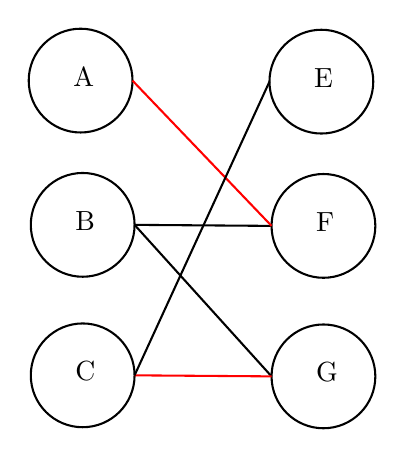
\begin{tikzpicture}[x=0.75pt,y=0.75pt,yscale=-1,xscale=1]
%uncomment if require: \path (0,480); %set diagram left start at 0, and has height of 480

%Shape: Circle [id:dp8182178753611458] 
\draw   (92,74) .. controls (92,60.19) and (103.19,49) .. (117,49) .. controls (130.81,49) and (142,60.19) .. (142,74) .. controls (142,87.81) and (130.81,99) .. (117,99) .. controls (103.19,99) and (92,87.81) .. (92,74) -- cycle ;
%Shape: Circle [id:dp22627546770204] 
\draw   (208,74.5) .. controls (208,60.69) and (219.19,49.5) .. (233,49.5) .. controls (246.81,49.5) and (258,60.69) .. (258,74.5) .. controls (258,88.31) and (246.81,99.5) .. (233,99.5) .. controls (219.19,99.5) and (208,88.31) .. (208,74.5) -- cycle ;
%Shape: Circle [id:dp25237914516171434] 
\draw   (93,143.5) .. controls (93,129.69) and (104.19,118.5) .. (118,118.5) .. controls (131.81,118.5) and (143,129.69) .. (143,143.5) .. controls (143,157.31) and (131.81,168.5) .. (118,168.5) .. controls (104.19,168.5) and (93,157.31) .. (93,143.5) -- cycle ;
%Shape: Circle [id:dp10721429744261579] 
\draw   (209,144) .. controls (209,130.19) and (220.19,119) .. (234,119) .. controls (247.81,119) and (259,130.19) .. (259,144) .. controls (259,157.81) and (247.81,169) .. (234,169) .. controls (220.19,169) and (209,157.81) .. (209,144) -- cycle ;
%Shape: Circle [id:dp47831765680042193] 
\draw   (93,216) .. controls (93,202.19) and (104.19,191) .. (118,191) .. controls (131.81,191) and (143,202.19) .. (143,216) .. controls (143,229.81) and (131.81,241) .. (118,241) .. controls (104.19,241) and (93,229.81) .. (93,216) -- cycle ;
%Shape: Circle [id:dp26348558107546327] 
\draw   (209,216.5) .. controls (209,202.69) and (220.19,191.5) .. (234,191.5) .. controls (247.81,191.5) and (259,202.69) .. (259,216.5) .. controls (259,230.31) and (247.81,241.5) .. (234,241.5) .. controls (220.19,241.5) and (209,230.31) .. (209,216.5) -- cycle ;
%Straight Lines [id:da026513665416650234] 
\draw [color={rgb, 255:red, 0; green, 0; blue, 0 }  ,draw opacity=1 ]   (143,143.5) -- (209,216.5) ;
%Straight Lines [id:da3886449137592256] 
\draw [color={rgb, 255:red, 255; green, 0; blue, 0 }  ,draw opacity=1 ]   (143,216) -- (209,216.5) ;
%Straight Lines [id:da560956275992279] 
\draw [color={rgb, 255:red, 0; green, 0; blue, 0 }  ,draw opacity=1 ]   (143,143.5) -- (209,144) ;
%Straight Lines [id:da9678739558151976] 
\draw [color={rgb, 255:red, 255; green, 0; blue, 0 }  ,draw opacity=1 ]   (142,74) -- (209,144) ;
%Straight Lines [id:da0796239005962387] 
\draw [color={rgb, 255:red, 0; green, 0; blue, 0 }  ,draw opacity=1 ]   (143,216) -- (208,74.5) ;

% Text Node
\draw (112,66) node [anchor=north west][inner sep=0.75pt]   [align=left] {A};
% Text Node
\draw (228,66.5) node [anchor=north west][inner sep=0.75pt]   [align=left] {E};
% Text Node
\draw (113,135.5) node [anchor=north west][inner sep=0.75pt]   [align=left] {B};
% Text Node
\draw (229,136) node [anchor=north west][inner sep=0.75pt]   [align=left] {F};
% Text Node
\draw (113,208) node [anchor=north west][inner sep=0.75pt]   [align=left] {C};
% Text Node
\draw (229,208.5) node [anchor=north west][inner sep=0.75pt]   [align=left] {G};


\end{tikzpicture}
